\documentclass[letterpaper]{article}
\usepackage{amsmath,amssymb,graphicx}
\usepackage{color,soul}
\usepackage[dvipsnames]{xcolor}
\usepackage{hyperref}
\usepackage[ruled,linesnumbered]{algorithm2e}
\usepackage[font=small,skip=4pt]{caption}
\usepackage{subcaption}
\usepackage{csquotes}
\usepackage{pdfpages}
\usepackage{minted}
\setminted[python]{
  breaklines=true,
  frame=lines,
  framerule=0pt,
  framesep=0pt,
  linenos,
  fontsize=\small,
  mathescape,
}

\addtolength{\oddsidemargin}{-.875in}
\addtolength{\evensidemargin}{-.875in}
\addtolength{\textwidth}{1.75in}
\addtolength{\topmargin}{-1.50in}
\addtolength{\textheight}{2.5in}


\hypersetup{
  colorlinks,
  linkcolor={MidnightBlue},
  citecolor={blue},
  urlcolor={MidnightBlue}
}

\usepackage{hyperref}

% Example definitions.
% --------------------
% nice symbols for real and complex numbers
\newcommand{\R}[0]{\mathbb{R}}
\newcommand{\C}[0]{\mathbb{C}}
\newcommand{\TODO}{\hl{\textbf{TODO}}}
\newcommand{\INPROGRESS}{\sethlcolor{cyan}\hl{\textbf{INPROGRESS}}\sethlcolor{yellow}}
\newcommand{\comment}[1]{\textcolor{OliveGreen}{#1}}

% definitions from Variational inference: A review for statisticians
\newcommand{\red}[1]{\textcolor{BrickRed}{#1}}
\newcommand{\orange}[1]{\textcolor{BurntOrange}{#1}}
\newcommand{\green}[1]{\textcolor{OliveGreen}{#1}}
\newcommand{\blue}[1]{\textcolor{MidnightBlue}{#1}}
\newcommand{\magenta}[1]{\textcolor{RubineRed}{#1}}
\newcommand{\teal}[1]{\textcolor{TealBlue}{#1}}
\newcommand{\gray}[1]{\textcolor{black!60}{#1}}

\DeclareRobustCommand{\mb}[1]{\ensuremath{\boldsymbol{\mathbf{#1}}}}

\DeclareMathOperator*{\argmax}{arg\,max}
\DeclareMathOperator*{\argmin}{arg\,min}

\DeclareMathOperator*{\diag}{diag}

\newcommand\dif{\mathop{}\!\mathrm{d}}

\newcommand{\bm}{\mathbf{m}}
\newcommand{\bs}{\mathbf{s}}

\newcommand{\bw}{\mathbf{w}}
\newcommand{\bx}{\mathbf{x}}
\newcommand{\by}{\mathbf{y}}
\newcommand{\bz}{\mathbf{z}}
\newcommand{\balpha}{\mb{\alpha}}
\newcommand{\bbeta}{\mb{\beta}}
\newcommand{\bmu}{\mb{\mu}}
\newcommand{\bsigma}{\mb{\sigma}}
\newcommand{\btheta}{\mb{\theta}}
\newcommand{\blambda}{\mb{\lambda}}
\newcommand{\bgamma}{\mb{\gamma}}
\newcommand{\bphi}{\mb{\phi}}
\newcommand{\btau}{\mb{\tau}}
\newcommand{\bvarphi}{\mb{\varphi}}
\newcommand{\bc}{\mathbf{c}}
\newcommand{\ELBO}{\textsc{elbo}}
\newcommand{\cN}{\mathcal{N}}
\newcommand{\cQ}{\mathcal{Q}}

\newcommand{\g}{\,\vert\,}
\newcommand{\E}{\mathbb{E}}
\newcommand{\EE}[1]{\mathbb{E}\left[#1\right]}
\newcommand{\EEE}[2]{\mathbb{E}_{#1}\left[#2\right]}
\newcommand{\grad}{\nabla}
\newcommand{\gradd}[1]{\nabla_{#1}}
\newcommand{\kl}[1]{\textsc{kl}\left(#1\right)}
\newcommand{\vct}[1]{\textbf{#1}}
\newcommand{\realline}{\mathbb{R}}
\newcommand{\indpt}{\protect\mathpalette{\protect\independenT}{\perp}}
\def\independenT#1#2{\mathrel{\rlap{$#1#2$}\mkern2mu{#1#2}}}
\newcommand{\h}[1]{\textrm{H}\left( #1 \right)}
\newcommand{\half}{\frac{1}{2}}
\newcommand{\new}{\textrm{new}}
\newcommand{\mult}{\textrm{Mult}}
\newcommand{\Dir}{\textrm{Dir}}
\newcommand{\discrete}{\textrm{Discrete}}
\newcommand{\Bern}{\textrm{Bern}}
\newcommand{\DP}{\textrm{DP}}
\newcommand{\GP}{\textrm{GP}}
\newcommand{\Bet}{\textrm{Beta}}
\newcommand{\const}{\mathrm{const}}
\newcommand{\pois}{\textrm{Pois}}

\newcommand{\ddx}[1]{\frac{\partial}{\partial #1}}
\newcommand{\dfdx}[2]{\textstyle \frac{\partial #1}{\partial #2}}

\newcommand{\yrep}{y^{\textrm{rep}}}
\newcommand{\ynew}{y^{\textrm{new}}}
\newcommand{\yobs}{y^{\textrm{obs}}}
\newcommand{\model}{\mathcal{M}}
\newcommand{\ppc}{\textrm{ppc}}
\newcommand{\ideal}{\textrm{ideal}}
\newcommand{\loglik}{\mathcal{L}}
\newcommand{\nw}{\textrm{new}}
\newcommand{\data}{\mathcal{D}}

\newcommand{\Gam}{\textrm{Gam}}

% bold paragraph titles
\newcommand{\mypar}[1]{{\bf #1.}}

\title{
  {\bf title of the big homework }\\
  \large Big homework in big course }
\author{Saurav Shekhar, (16-947-921)\\
  \href{mailto:shekhars@student.ethz.ch}{shekhars@student.ethz.ch}}
\date{\today}

\begin{document}
%  \tableofcontents
  \maketitle
  \begin{abstract}
    All notes regarding my masters thesis project
  \end{abstract}
  
  \section{External links}
  \begin{itemize}
    \item \href{https://docs.google.com/document/d/1GMczTKs5-JKIgxfFOKv1yJNKLoUHZ0pqwR15xZcgyYQ/edit?usp=sharing}{Thesis pre proposal}
    \item \href{https://docs.google.com/document/d/1Ytcuj1QJ8Xs5gzXVYbvcsjwsGGyz7HEg0_nCRAXjbgg/edit}{Tasks document}
    \item \href{https://gitlab.ethz.ch/shekhars/msc-thesis}{Gitlab repository} \comment{might be removed}
    \item \href{https://www.overleaf.com/9925566564xbszbcfbycnd}{Overleaf project} \comment{not regularly updated}
  \end{itemize}
  
  \section{Literature notes}
  
  \mypar{Variational inference}: \cite{blei2016variational} \INPROGRESS \\
  \begin{align}
    \blue{\overbrace{\kl{q(\bz)||p(\bz|\bx)}}^{\downarrow\text{ Objective } \geq 0} } &:= 
    \EEE{q(\bz)}{\log q(\bz)} - \EEE{q(\bz)}{\log p(\bz | \bx)} \\
    \text{ELBO}(q) &:= \EEE{q(\bz)}{\log p(\bz, \bx)} - \EEE{q(\bz)}{\log q(\bz)} \\
    \kl{q(\bz)||p(\bz|\bx)} + \magenta{\underbrace{\text{ELBO}(q)}_{\uparrow \text{Optimize}}}
     &= \underbrace{\log p(\bx)}_{\text{constant w. } q} \\
     \text{ELBO}(q) &= \EE{\log p(\bx | \bz)} - \kl{q(\bz) || p(\bz)} \\
     \text{ELBO}(q) &= \cQ(\theta, \theta_t) - \mathcal{H}(\bz|\bx) \text{ \comment{ //Entropy}}\\
  \end{align}
  \begin{algorithm}[h]
    \KwIn{A model $p(\bx, \bz)$, a data set $\bx$}
    \KwOut{A variational density $q(\bz) = \prod_{j=1}^{m} q_{j}(z_j)$}
    \textbf{Initialize:} Variational factors $q_{j}(z_j)$ \\
    \While{the ELBO has not converged} {
      \For{$j \in \{1, \ldots, m\}$} {
        Set $q_{j}(z_j) \propto \exp\{\E_{-j}[\log p(z_j \g \bz_{-j}, \bx)]\}$\\
        }
        Compute $\ELBO(q) = \EE{\log p(\bz, \bx)} - \EE{\log q(\bz)}$
        }
  \Return{$q(\bz)$}
  \caption{Coordinate Ascent for VI}
  \label{alg:cavi}
 \end{algorithm}
      
  \mypar{Exponential families conditional conjugacy} \cite{pgmai18}
  \TODO define conditional conjugacy properly
  \begin{algorithm}[h]
    \KwIn{A model $p$, variational family $q_{\phi(z)}, q_{\lambda}(z)$}
    \While{\text{ELBO is not converged}} {
      \For{\text{each data point} i} {
          Update $\varphi_i \gets \EEE{\lambda}{\eta_l(\beta, x_i)}$\\
        }
        Update $\lambda \gets \EEE{\varphi}{\eta_g(x, z)}$\\
      }
    \caption{VI with conjugate family assumption}
    \label{alg:vi_conj}
  \end{algorithm}

  \mypar{Gradient Optimization for ELBO}
  We will try to solve the optimization problem from Gradient ascent perspective.
  This will open up opportunity for stochastic optimization \cite{robbins1951stochastic}
  \cite{robbins1985stochastic}.
  
  Moving from Gradient Opt to Stochastic VI
  \begin{enumerate}
    \item subsample a data point $t$ from full data
    \item use current global param $\lambda$ to update local param $\varphi_t$
    \item update $\lambda$
  \end{enumerate}

  Gradient optimization step $\lambda_{t + 1} = \lambda_{t} + \delta\nabla_{\lambda}f(\lambda_{t})$.
  An equivalent formulation (for small $d\lambda$) is
  \begin{align}
   \argmax_{d\lambda} f(\lambda + d\lambda) \text{ st. } ||d\lambda||^2 \leq \epsilon
  \end{align}

  Here we have euclidean distance metric, which is not the best choice for 
  probability distributions. For ex - $q_{\lambda} \sim \cN(0, 1000)$ is much closer
  distribution to $q_{\lambda{''}} \sim \cN(10, 10000)$ than $q_{\lambda{'}} \sim \cN(0, 0.001)$
  is to $q_{\lambda{'''}}\cN(0.1, 0.001)$ even though $||\lambda - \lambda{''}|| \geq ||\lambda{'} - \lambda{'''}||$

  {\bf Natural gradient of ELBO}: \emph{natural gradient} accounts for geometric
  structure of probability parameters ($\lambda$). They wrap the parameter space
  in a sensible way such that moving in same direction in different directions
  amounts to equal change in symmetrized KL divergence.

  \begin{align}
    \argmax_{d\lambda} f(\lambda + d\lambda) \text{ st. } \\\nonumber
    D^{sym}_{KL}(q_{\lambda}, q_{\lambda + d\lambda}) \leq \epsilon \text{ where } \\\nonumber
    D^{sym}_{KL}(q, p) = KL(q||p) + KL(p||q)
  \end{align}

  We need to find Riemannian metric \footnote{seems to be some kind of transformation}
  $G(\lambda)$ which transforms euclidean distance to symmetrized KL divergence:
  \begin{align}
    d\lambda^\intercal d\lambda = D^{sym}_{KL}(q_{\lambda}(\beta), q_{\lambda + d\lambda}(\beta))
  \end{align}
  Using information geometry \footnote{Hope so}, we can also rescale the gradients
  in the right space:
  \begin{align}
    \label{eqn:g_inv_eqn}
    \hat{\nabla_{\lambda}}ELBO &= G^{-1}(\lambda)\nabla_{\lambda}ELBO \text{ where } \\
    G(\lambda) &= \EE{{\Big(\nabla_{\lambda} \log q_{\lambda} (\beta) \Big)}
                      {\Big(\nabla_{\lambda} \log q_{\lambda} (\beta) \Big)}^\intercal}
                    \label{eqn:g_fis_inf}
  \end{align}
  $G(\lambda)$ is the Fisher information matrix. For our model class (conjugate exponential...)
  We've
  \begin{align} \label{eqn:gradq}
    \nabla_{\lambda} \log q_{\lambda} (\beta) = t(\beta) - \EE{t(\beta)}
  \end{align}
  Combining \ref{eqn:gradq} and \ref{eqn:g_fis_inf}
  \begin{align}
    G(\lambda) = \nabla_{\lambda}^{2}a(\lambda) = a{''}(\lambda) \label{eqn:g_dd}
  \end{align}
  From \cite{hoffman2013stochastic}, equation of Euclidean gradient
  \begin{align}
    \nabla_{\lambda}ELBO = a{''}(\lambda)\Big(\EE{\eta(\bx, \bz)} - \lambda\Big)
    \label{eqn:elbo_euc_grad}
  \end{align}
  \TODO \comment{refresh \ref{eqn:elbo_euc_grad} with value in \cite{blei2016variational}} \\
  Combining \ref{eqn:g_inv_eqn}, \ref{eqn:elbo_euc_grad} and \ref{eqn:g_dd}
  \begin{align}
    g(\lambda) = \widehat{\nabla_{\lambda}}ELBO &= \EE{\eta(\bx, \bz)} - \lambda \text{ and } \nonumber\\
    \lambda_t &= \lambda_{t - 1} + \delta_t g(\lambda_{t - 1}) \nonumber\\
    \Rightarrow \lambda_t &= (1 - \delta_t)\lambda_{t - 1} +  \delta_t  \EE{\eta(\bx, \bz)} 
  \end{align}
  \begin{algorithm}[h]
  \KwIn{A model $p$, variational family $q_{\phi(z)}, q_{\lambda}(z)$}
  \While{\text{ELBO is not converged}} {
    \For{\text{each data point} i} {
      Update $\varphi_i \gets \EEE{\lambda}{\eta_l(\beta, x_i)}$\\
    }
    \red{Update $\lambda \gets (1 - \delta_t)\lambda +
                                  \delta_t \EEE{q(\varphi)}{\eta_g(x, z)}$}\\
  }
  \caption{VI with conjugate family assumption}
  \label{alg:vi_nat_grad}
  \end{algorithm}
  
  \mypar{Stochastic Variational inference}
  in Algorithm \ref{alg:vi_nat_grad} line 2-4, we have to iterate over all data 
  to compute the new set of local variables $\varphi$. This does not scale well
  to large datasets. \cite{hoffman2013stochastic}
  So we have to use stochastic gradients. Noisy gradients $H$ of $f$ will converge
  to a local optimum as long as
  \begin{itemize}
    \item $\EE{H} = \nabla f$
    \item Step size $\delta_t$ st: $\sum_{1}^{\infty}\delta_t = \infty$ and
    $\sum_{1}^{\infty}\delta_t^{2} < \infty$
  \end{itemize}
  Now,
  $$
    \EE{\eta(\bx, \bz)} = \Big(\alpha_1 + \sum_{1}^{n}\EEE{q}{t(z_i, x_i)},
                               n + \alpha_2 \Big)
  $$
  Noisy gradient by sampling
  \begin{enumerate}
    \item Sample $t \sim Uniform(1, \ldots, n)$
    \item Rescale 
      \begin{align*}
        g(\lambda) &= \Big(\alpha_1 + n\EEE{q}{t(z_t, x_t)},
                      n + \alpha_2 \Big) - \lambda \\
                   &=: \hat{\lambda} - \lambda
      \end{align*}
  \end{enumerate}
  \begin{algorithm}[h]
  \KwIn{A model $p(\bx, \bz)$, data $\bx$}
  {\bf Initialize:}{variational family $q_{\phi(z)}, q_{\lambda}(z)$ with params $\lambda_{0}$}\\
  \KwResult{Global variational densities $q_{\lambda}(\beta)$}
  \While{Stopping criteria not met} {
    \red{Sample $t \sim Uniform(1, \ldots, n)$} \\
    \red{Update $\phi_t \gets \EEE{\lambda}{\eta_l(\beta, x_t)}$} \\
    \red{Compute global param estimate $\hat{\lambda} = \EEE{\varphi}{\eta_g(z_t, x_t)}$} \\
    \red{Update $\lambda \gets (1 - \delta_t)\lambda +
            \delta_t \hat{\lambda}$} \\
  }
  \Return{$\lambda$}
  \caption{Stochastic VI}
  \label{alg:vi_stoc_grad}
  \end{algorithm}

  Research on optimizing difficult variational objectives with Monte Carlo (MC)
  estimates. Write gradient of ELBO as expectation, compute MC estimates, use stochastic
  optimization with MC estimates. New approaches avoid any model-specific derivations,
  and are called 'Black-box' inference techniques. As examples, see - \cite{kingma2013auto}
  \cite{rezende2014stochastic} \cite{ranganath2014black} \cite{ranganath2016hierarchical}
  \cite{titsias2014doubly} \cite{kucukelbir2017automatic}

  $$
    \text{ELBO} = \EEE{q_{\nu}}{\log p_{\theta}(z, x)} - \EEE{q}{\log q_{\nu}{z}}
  $$
  $\nu$ params of variational family, $\theta$ params of model. We need unbiased estimates
  of $\nabla_{\nu, \theta}ELBO$ to maximize ELBO.
  
  \mypar{Black Box variational inference} \INPROGRESS \\
    From \cite{ranganath2014black}
    \begin{displayquote}
      We will form the derivative of the objec-
      tive as an expectation with respect to the variational
      approximation and then sample from the variational ap-
      proximation to get noisy but unbiased gradients, which
      we use to update our parameters. For each sample, our
      noisy gradient requires evaluating the joint distribution
      of the observed and sampled variables, the variational
      distribution, and the gradient of the log of the varia-
      tional distribution. This is a black box method in that
      the gradient of the log of the variational distribution
      and sampling method can be derived once for each type
      of variational distribution and reused for many models
      and applications.
    \end{displayquote}
    \begin{displayquote}
       \red{We will form the $\nabla ELBO$ as an $\EEE{q_\lambda}{...}$ 
       and then sample $S$ samples from the $q_\lambda$ to get noisy but unbiased gradients (w.r.t $\lambda$), which
       we use to update $\lambda$. For each sample, our
       noisy gradient requires evaluating the $p(\bx, \bz_{S}), q(\bz_{S})$, and
        $\nabla \log q(\bz_{S})$. This is a black box method in that
       the $\nabla \log q(\bz_{S})$
       and sampling method can be derived once for each type
       of variational distribution and reused for many models
       and applications.}
    \end{displayquote}
  Equation (2) of \cite{ranganath2014black}
  \begin{align}
    \nabla_{\lambda}\mathcal{L} &= \EEE{q}{\nabla_{\lambda}\log q(z|\lambda) \Big(\log p(x, z) - \log q(z|\lambda\Big)} \label{eqn:bbvi_grad} \text{ where } \\
    \mathcal{L}(\lambda) &\overset{\triangle}{=}  \EEE{q_{\lambda_{z}}}{\log p(x, z) - \log q(z)} \text{ (ELBO) } \nonumber
  \end{align}
  \comment{\href{https://github.com/hoangcuong2011/Good-Papers/blob/master/Black\%20Box\%20Variational\%20Inference.md}{here} it says that Equation 2/3 can be derived simply using the
  log trick but the authors use a complicated method in paper. Also derived in \cite{pml18}}
  and \cite{pgmai18}\\
  the gradient $\nabla_{\lambda}\log q(z|\lambda)$ of the log of a probability distribution
  is called the score function or REINFORCE \\
  Basic algorithm
   \begin{flalign}
    z_s &\sim q(z|\lambda) \text{ for } s \in {1..S} \nonumber\\
    \nabla_{\lambda}\mathcal{L} &\approx \frac{1}{S} \sum_{s=1}^{S} \nabla_{\lambda}\log q(z_s | \lambda) 
                      \Big(\log p(x, z_s) - \log q(z_s|\lambda)\Big)
   \end{flalign}
  Rao-Blackwellization and smart Control Variates to control variance\\
  \comment{Variance still very high. Reparameterization and amortization come to rescue (See
  \href{https://www.youtube.com/watch?v=Dv86zdWjJKQ}{this} tutorial from David Blei)}
  
  \comment{Good notes on 
   \href{http://www.it.uu.se/research/systems_and_control/education/2018/pml/lectures/VILectuteNotesPart2.pdf}{Stochastic VI}
  and \href{http://www.it.uu.se/research/systems_and_control/education/2018/pml/lectures/VILectuteNotesPart3.pdf}{Black Box VI} from \cite{pml18}} \\

  \mypar{Reparameterization trick} 
  \\\TODO
  
  \mypar{Boosting Variational inference}
    \TODO

  \mypar{Frank-Wolfe} \INPROGRESS
    \cite{jaggi2013revisiting} \cite{pedregosa2018frank} 
    \cite{pedregosa2018step} \cite{doi:10.1002/zamm.19730530723}
  \begin{algorithm}[h]
    \textbf{Constrained Optimization:} $\min\limits_{x \in \data} f(\bx)$ \\
    \For{$t \in \{0, \ldots, T\}$} {
      $s^t \gets \argmin_{s \in \data}\langle \bs, \grad f(\bx^{t}) \rangle$ \\
      $\bx^{t + 1} \gets \mathbf{UpdateRule}(\bx^t, s^t, t, f)$
    }
  \caption{Frank-Wolfe}
  \label{alg:fw}
 \end{algorithm}
 \comment{Here $x, \mathcal{D} \equiv x, \mathcal{D} \equiv q, \mathcal{A}$}\\
 $\mathbf{UpdateRule}$ can be
 \begin{align}
   q^{t + 1} &\gets (1 - \gamma) q^t + \gamma s^t = q^t + \gamma\overbrace{(s^t - q^t)}^{d_t} 
 \textrm{ where}\nonumber\\
 \mathbf{Variant 0:} 
   \gamma &\gets \frac{2}{t + 2} \\
 \mathbf{Variant 1:}
   \gamma &\gets \argmin\limits_{\gamma \in [0, 1]} f((1 - \gamma) q^t + \gamma s^t)
    \label{eqn:update_lsearch} \\
  g_t &\gets -\langle \grad f(\bx_t), d_t \rangle \rangle \nonumber\\
 \mathbf{Exit condition:} g_t &< \delta \nonumber\\
 \mathbf{Variant 2:} \gamma &\gets \min \Big(\frac{g_t}{L ||d_t|| ^2}, 1\Big)
 \label{eqn:var2_update} \\
 \mathbf{Variant 3:} \nonumber\\
   q^{t + 1} &\gets \argmin\limits_{q \in \bigcup_{i=1}^{t}{s^t}}f(q) \nonumber\\
 \end{align}
 \ref{eqn:var2_update} has variants \cite{pedregosa2018frank} \cite{Demyanov70} \TODO add more
 \red{$$
 \gamma \gets \min \Big\{\frac{g_t}{L\text{ diam}(\data) ^2}, 1\Big\}
 \label{eqn:var2b} \\
 $$}

  \mypar{Boosting Black Box Variational inference} \INPROGRESS \\
  Boosting introduced in \cite{guo2016boosting}, connection with FW in \cite{locatello2017boosting}.
  define a Linear Minimization Problem (LMO) as
  $
  \mathbf{LMO}_{\mathcal{A}}(y) := \argmin\limits_{s \in \mathcal{A}} \langle y, s \rangle
  $
  In line 3 of \ref{alg:fw}, rewrite it as
  $$
  s^t \gets (\delta-\text{Approx-})\mathbf{LMO}_{\mathcal{A}}(\grad f(q^t))
  $$
  Algorithm for LMO in section 4 of \cite{locatello2018boosting}. In Theorem 2,
  Curvature $\mathcal{C}_{f,\mathcal{A}}$ is bounded for $D^{KL}$ if param. space of
  densities in $\mathcal{A}$ is bounded. In section 3, a bounded curvature for
   $D^{KL}$ is obtained.
   
  {\bf Black box LMO}: \\
  \comment{In this case $f(q^t) = \kl{q^t(\bz) || p(\bx, \bz)}$ }. Assuming 
  $\theta$ are the parameters defining variational family $\mathcal{Q} \equiv \mathcal{A}$
  We've to find $\gradd{\theta}f(q^t)$, more specifically, we've to find 
  $$
  s^t \gets (\delta-\text{ Approx.}) \argmin\limits_{s \in \mathcal{A}}\langle 
    \grad \kl{q^t(\bz) || p(\bx, \bz)}, s \rangle
  $$
  \TODO add how \cite{guo2016boosting} \cite{locatello2017boosting} deal with optimization of LMO. Also
  add the part about $\text{conv}(\mathcal{A})$ being sufficient instead of $\mathcal{A}$.\\
  Convergence of SGD not fully understood. To guarantee convergence of FW, solution of LMO should 
  not be degenerate. This translates to a constraint on $||s||_{\infty}$ which is not practical.
  Every pdf with bounded $||\cdot||_{\infty}$ has bounded entropy and the converse holds true in 
  most cases of interest. \comment{(Gaussian, Laplacian, ...)}. Assume $\mathcal{A}$ is such a family
  and $\bar{\mathcal{A}}$ is $\mathcal{A}$ w/o $l_{\infty}$ norm constraint.  \TODO ask
  $$
  \argmin\limits_{s \in \bar{\mathcal{A}}, \mathcal{H}(s) \geq -M}\langle \grad 
  \kl{q^t(\bz) || p(\bx, \bz)},
  s \rangle \orange{\overset{?}{\equiv}}
    \argmin\limits_{s \in \bar{\mathcal{A}}, \mathcal{H}(s) \geq -M}\Big\langle s, 
    \log \frac{q^t}{p} \Big\rangle
  $$
  Using Lagrange multiplier $\lambda$
  \begin{align}
    \Bigg\langle s, \log \Big(\frac{s}{\sqrt[\lambda]{\frac{p}{q^t}}} \Big)\Bigg\rangle \nonumber\\
      &\equiv \argmin\limits_{s \in \bar{\mathcal{A}}}\kl{s||{\sqrt[\lambda]{\frac{p}{q^t}}} Z} \nonumber\\
    \text{RELBO}(s, \lambda) &:= \EEE{s}{\log p} - \EEE{s}{\log q^t} - \lambda\EEE{s}{\log s}
  \end{align}
  For true LMO solution, will need to maximize for $\lambda$. Might end in saddle, fix or slowly decrease
  with time $\frac{1}{\sqrt{t + 1}}$

  \section{Ideas}
  \subsection{Line search}
  Line search in \ref{eqn:update_lsearch} is not working very well. 
  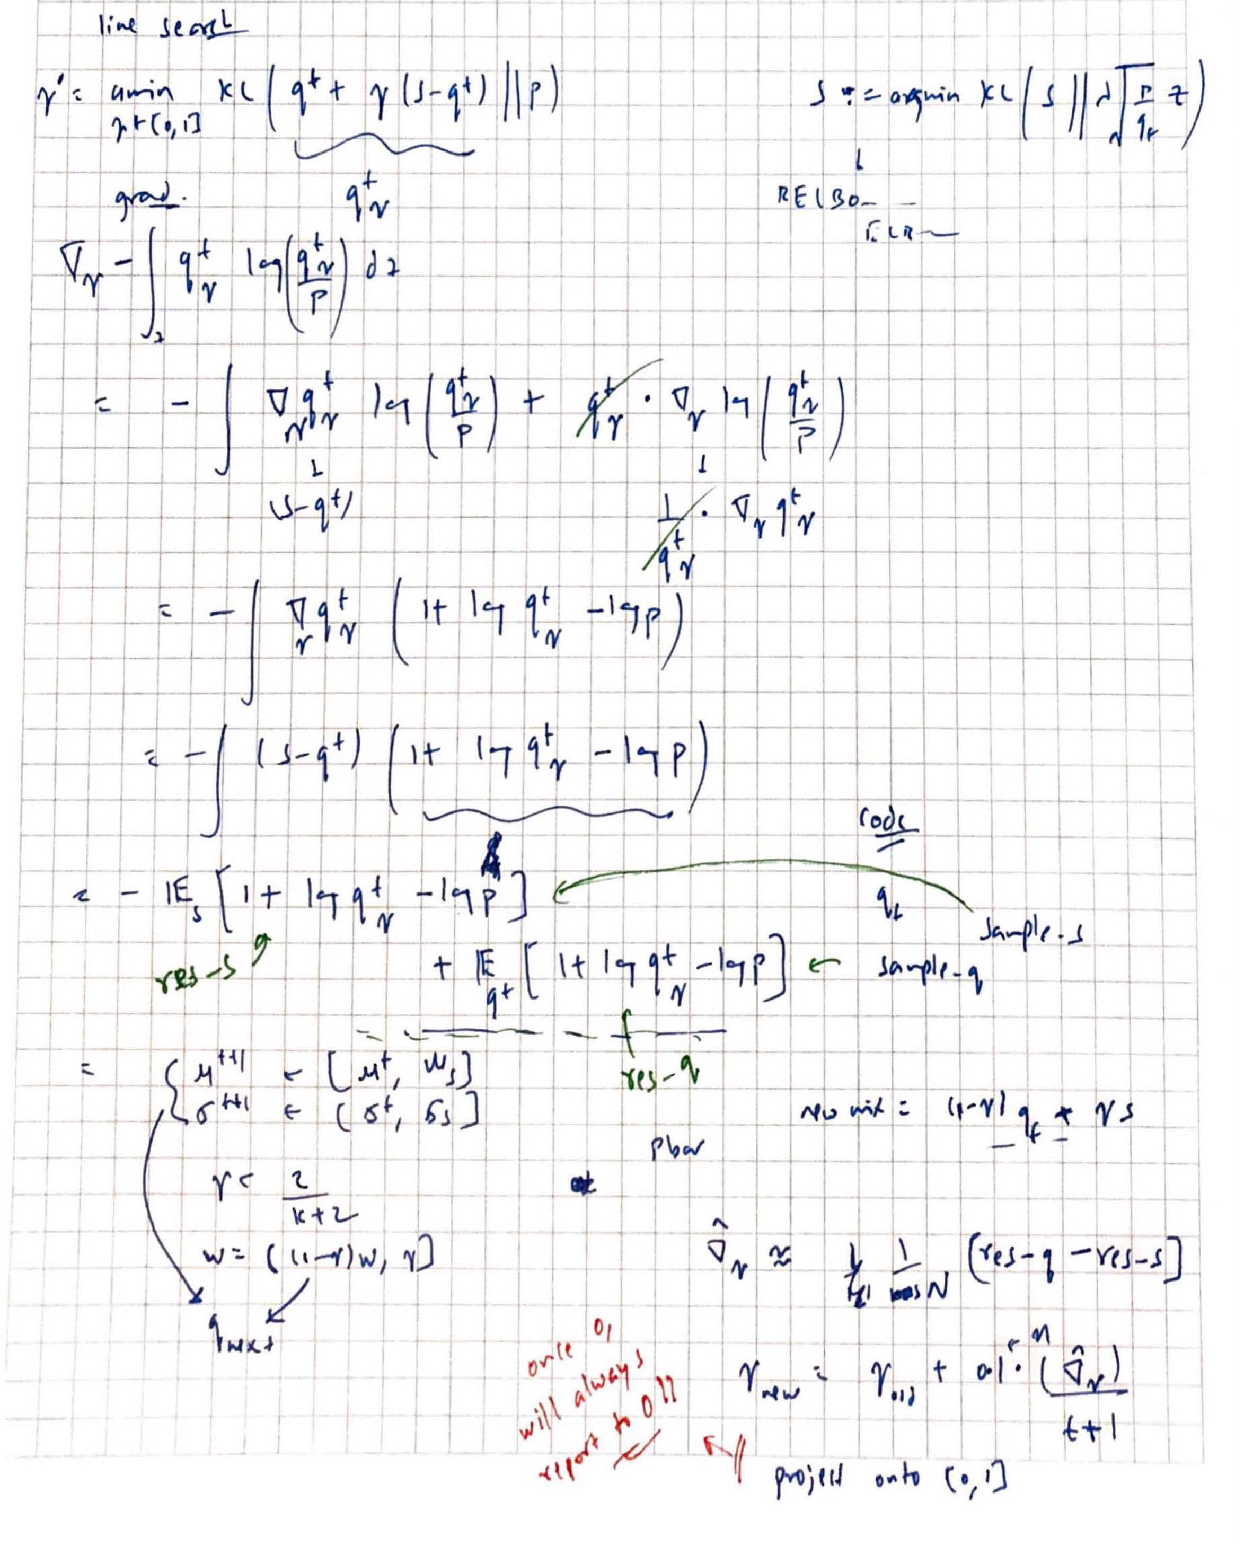
\includepdf{Thesis_notes_Nov_1.pdf}
  %\inputminted[firstline=140,lastline=220,mathescape]{python}
  %  {../boosting_bbvi/scripts/mixture_model_relbo.py}
  \begin{minted}{python}
def line_search_dkl(weights, locs, diags, mu_s, cov_s, x, k):
    """Perform line search for the best step size gamma.
    
    Uses gradient ascent to find gamma that minimizes
    KL(q_t + gamma (s - q_t) || p)
    
    Args:
        weights: weights of mixture components of q_t
        locs: means of mixture components of q_t
        diags: deviations of mixture components of q_t
        mu_s: mean for LMO Solution s
        cov_s: cov matrix for LMO solution s
        x: target distribution p
        k: iteration number of Frank-Wolfe
    Returns:
       Computed gamma
    """
    def softmax(v):
        return np.log(1 + np.exp(v))
    # no. of samples to approximate $\nabla_{\gamma}$
    N_samples = 10
    # Create current iter $q_t$
    weights = [weights]
    qt_comps = [
        Normal(
            loc=tf.convert_to_tensor(locs[i]),
            scale=tf.convert_to_tensor(diags[i])) for i in range(len(locs))
    ]
    qt = Mixture(
        cat=Categorical(probs=tf.convert_to_tensor(weights)),
        components=qt_comps,
        sample_shape=N)
    qt = InfiniteMixtureScipy(stats.multivariate_normal)
    qt.weights = weights[0]
    qt.params = list(
        zip([[l] for l in locs], [[softmax(np.dot(d, d))] for d in diags]))
    # samples from $q_t$
    sample_q = qt.sample_n(N_samples)
    # create and sample from s
    s = stats.multivariate_normal([mu_s],
                                  np.dot(np.array([cov_s]), np.array([cov_s])))
    sample_s = s.rvs(N_samples)
    # $q_{t+1}$ is mixture of $q_t$ and s with weights $(1 - \gamma)$ and $\gamma$
    # Set its corresponding parameters and weights
    new_locs = copy.copy(locs)
    new_diags = copy.copy(diags)
    new_locs.append([mu_s])
    new_diags.append([cov_s])
    # initialize $\gamma$
    gamma = 2. / (k + 2.)
    # no. steps of gradient ascent
    n_steps = 10
    prog_bar = ed.util.Progbar(n_steps)
    for it in range(n_steps):
        print("line_search iter %d, %.5f" % (it, gamma))
        new_weights = copy.copy(weights)
        new_weights[0] = [(1. - gamma) * w for w in new_weights[0]]
        new_weights[0].append(gamma)
        # create $q_{t + 1}^{\gamma}$
        q_next = InfiniteMixtureScipy(stats.multivariate_normal)
        q_next.weights = new_weights[0]
        q_next.params = list(
            zip([[l] for l in new_locs], [[np.dot(d, d)] for d in new_diags]))
        # Computes $\mathbb{E}[...] \propto \sum_{v}{\log p - \log q_{t + 1}^{\gamma}}$
        def px_qx_ratio_log_prob(v):
            Lambda = 1.
            ret = x.log_prob([v]).eval()[0] - q_next.log_prob(v)
            ret /= Lambda
            return ret
        # Samples w.r.t s
        rez_s = [
            px_qx_ratio_log_prob(sample_s[ss]) for ss in range(len(sample_s))
        ]
        # Samples w.r.t $q_{t+1}$
        rez_q = [
            px_qx_ratio_log_prob(sample_q[ss]) for ss in range(len(sample_q))
        ]
        # TODO(sauravshekhar) measure how noisy gradients are
        # Gradient ascent step, step size decreasing as $\frac{1}{it + 1}$
        gamma = gamma + 0.1 * (sum(rez_s) - sum(rez_q)) / (N_samples *
                                                           (it + 1.))
        # Projecting it back to [0, 1], too small range?
        # FIXME(sauravshekhar) if projected to 0, all iterations will be same?
        if gamma >= 1 or gamma <= 0:
            gamma = max(min(gamma, 1.), 0.)
            break
    return gamma
  \end{minted}
  \begin{figure}[h] \label{fig:gamma}
  \centering
  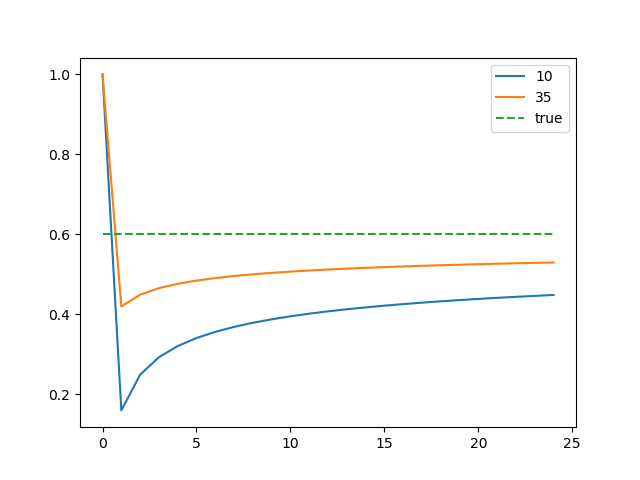
\includegraphics[width=0.9\textwidth]{plots/gamma.png}
  \caption{gamma with iterations for different n\_samples}
  \end{figure}
  \begin{figure}[h] \label{fig:es10}
    \centering
    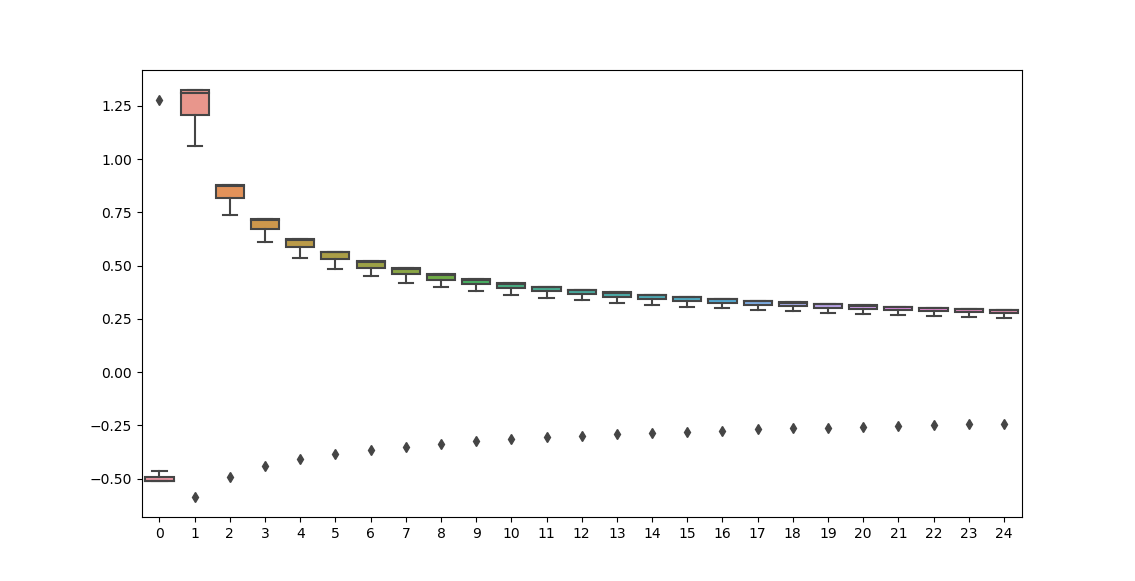
\includegraphics[width=0.9\textwidth]{plots/box_e_s_10.png}
    \caption{Boxplot for expectation w.r.t s for n\_samples = 10}
  \end{figure}
  \begin{figure}[h] \label{fig:es35}
  \centering
  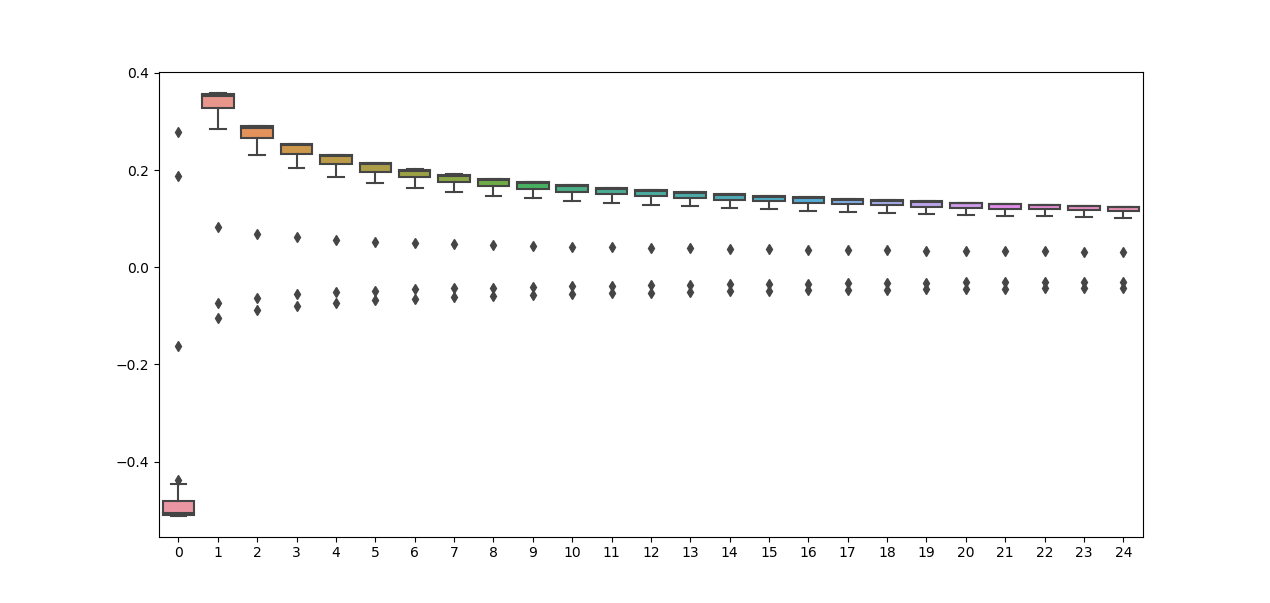
\includegraphics[width=0.9\textwidth]{plots/box_e_s_35.png}
  \caption{Boxplot for expectation w.r.t s for n\_samples = 36}
  \end{figure}
  \TODO make $E_q$ plot with iterations starting from 1
  \begin{figure}[h] \label{fig:eq10}
    \centering
    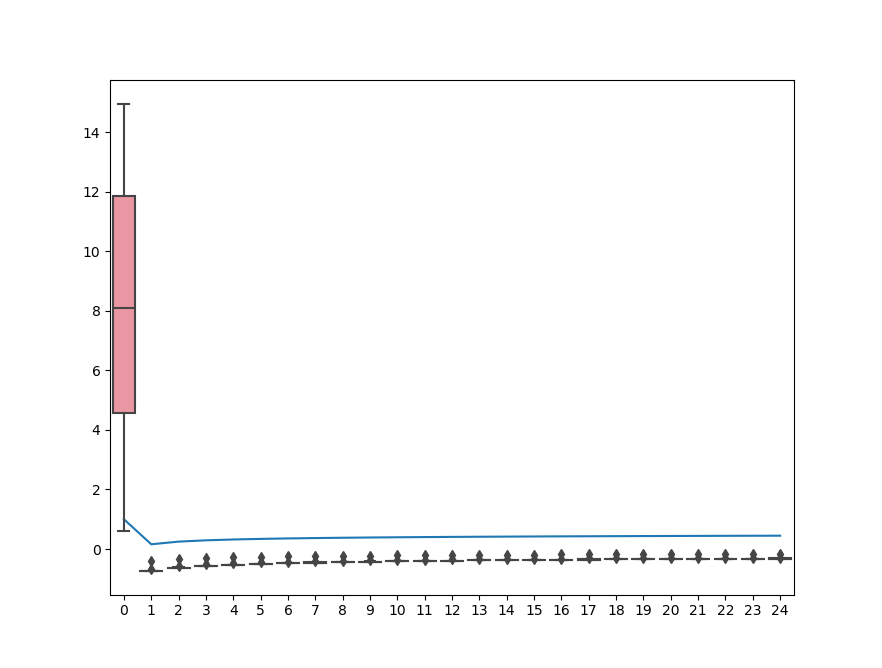
\includegraphics[width=0.9\textwidth]{plots/box_e_q_10.png}
    \caption{Boxplot for expectation w.r.t q\_t\^gamma for n\_samples = 10}
  \end{figure}
  \begin{figure}[h] \label{fig:eq35}
  \centering
  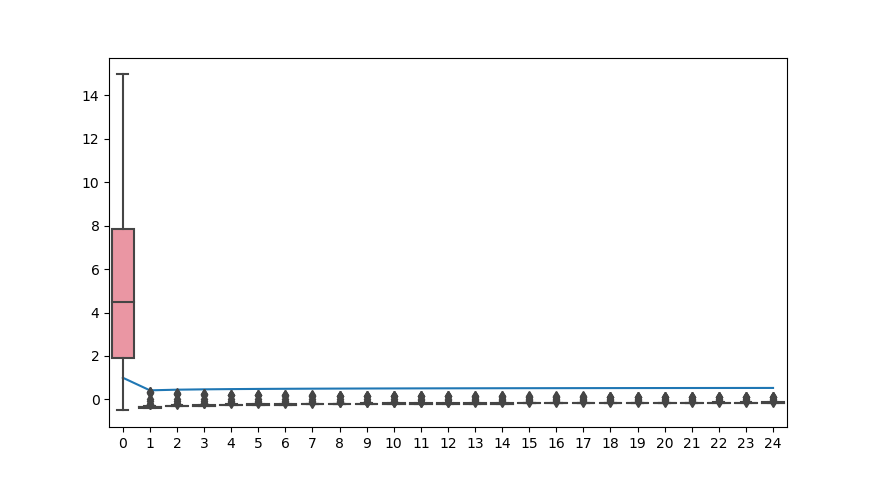
\includegraphics[width=0.9\textwidth]{plots/box_e_q_35.png}
  \caption{Boxplot for expectation w.r.t q\_t\^gamma for n\_samples = 35}
  \end{figure}
  \newpage
  \section{Math notes}
  \mypar{Shannon Entropy} \\
  Self information of event x $= x$ is defined as $I(x) := -\log P(x)$
  $$
  H(x) = \EEE{x \sim P}{I(x)} = -\EEE{x \sim P}{\log P(x)}
  $$
  \mypar{Cramer-Rao lower bound} \cite{math-stat16} 
  Suppose $\theta$ is an unknown deterministic parameter which is to be estimated from
  measurements $x$, distributed according to some pdf $f(x; \theta)$. The variance of any 
  \textit{unbiased estimator} $\hat{\theta}$ of $\theta$ is then bounded by reciprocal of
  Fischer Information $I(\theta)$:
  \begin{align}
    \text{var}(\hat{\theta}) &\geq \frac{1}{I(\theta)} \text{ where }\nonumber\\
    I(\theta) &= \EE{\Big(\frac{\partial l(x; \theta)}{\partial \theta}\Big)^2} \nonumber\\
         &= -\EE{\frac{\partial^2 l(x; \theta)}{\partial \theta^2}} \nonumber
  \end{align}
  {\bf Note}: See Wikipedia for other more general versions


  \newpage
  \section{Code Notes}
  Normal distribution edward

  \begin{minted}{python}
  from edward.models import Normal
  from keras.layers import Dense
  
  hidden = Dense(256, activation='relu')(x_ph)
  qz = Normal(loc=Dense(10)(hidden),
  scale=Dense(10, activation='softplus')(hidden))
  \end{minted}
  
  \newpage
  \bibliographystyle{apalike}
  \bibliography{refs}
 
  
 %$$
 %w_{t + 1} - w_{t} = \mu(w_t - w_{t - 1}) - \alpha_t \nabla_w f(w_t, z)
 %$$
  
  %\begin{table}[]
  %  \centering
  %  \parbox{\linewidth}{
  %    \begin{tabular}{c|c}
  %      OP & Latency  \\
  %      \hline
  %      mul & 5 \\
  %    \end{tabular}
  %    \caption{Mul}
  %    \label{tab:51}
  %  }  
  %\end{table}
  
  %\inputminted[firstline=1,lastline=200]{python}{code/boosting_bbvi/core/relbo.py}
\end{document}
